\documentclass{article}
\usepackage{fullpage,color,pgf,tikz}
\usepackage{authblk}
\title{Logic behind the bitsets used for updating diploids in multilocus simulations}
\author[1]{Kevin R. Thornton}
\affil[1]{Department of Ecology and Evolutionary Biology, UC Irvine}
\begin{document}
\maketitle

\begin{figure}[!h]
  \centering
  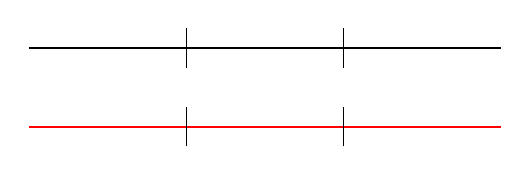
\begin{tikzpicture}
    % p1g1
    \path[draw,thick](0,1.5) -- (6,1.5);
    \path[draw](2,1.25)--(2,1.75); 
    \path[draw](4,1.25)--(4,1.75);
    
    % p1g2
    \path[draw,color=red,thick](0,0.5) -- (6,0.5);
    \path[draw](2,0.25)--(2,0.75); 
    \path[draw](4,0.25)--(4,0.75);
  \end{tikzpicture} 
  \caption{Multiple loci}
  \end{figure}
  

\begin{figure}[!h]
  \centering
  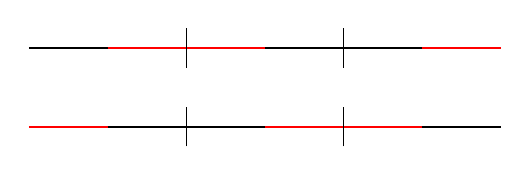
\begin{tikzpicture}
    % p1g1
    \path[draw,thick](0,1.5) -- (1,1.5);
    \path[draw,color=red,thick](1,1.5) -- (3,1.5);
    \path[draw,thick](3,1.5) -- (5,1.5);
    \path[draw,color=red,thick](5,1.5) -- (6,1.5);
    \path[draw](2,1.25)--(2,1.75); 
    \path[draw](4,1.25)--(4,1.75);
    
    % p1g2
    \path[draw,color=red,thick](0,0.5) -- (1,0.5);
    \path[draw,thick](1,0.5) -- (3,0.5);
    \path[draw,color=red,thick](3,0.5) -- (5,0.5);
    \path[draw,thick](5,0.5) -- (6,0.5);

    \path[draw](2,0.25)--(2,0.75); 
    \path[draw](4,0.25)--(4,0.75);
  \end{tikzpicture} 
  \caption{Odd number of crossovers within loci 0 and 1.  No crossover between the loci.}
\end{figure}

\end{document}
